\documentclass[tikz,border=8pt]{standalone}
\usepackage{ctex}
\usepackage{amsmath,amssymb}
\usetikzlibrary{arrows.meta,calc,angles,quotes,patterns,positioning,decorations.pathmorphing}
\definecolor{ink}{RGB}{30,43,58}
\definecolor{blue}{RGB}{38,92,168}
\definecolor{orange}{RGB}{220,112,24}
\definecolor{green}{RGB}{38,139,93}
\definecolor{red}{RGB}{192,53,53}
\tikzset{
 line cap=round,line join=round,
 body/.style={draw=ink,very thick},
 axis/.style={-{Latex[length=2.5mm]},draw=ink,very thick},
 vec/.style={-{Latex[length=2.5mm]},draw=blue,very thick},
 force/.style={-{Latex[length=2.5mm]},draw=red,very thick},
 guide/.style={draw=ink!48,dashed},
 dim/.style={{Latex[length=2mm]}-{Latex[length=2mm]},draw=ink!70}
}

\usetikzlibrary{decorations.pathmorphing}
\tikzset{mass/.style={circle,draw,fill=white,minimum size=7mm},curve/.style={very thick,blue},rope/.style={very thick,blue},ray/.style={very thick,blue,-{Latex}},impulse/.style={very thick,orange,-{Latex}},current/.style={very thick,orange,-{Latex}},resistor/.style={thick,decorate,decoration={zigzag,segment length=3mm,amplitude=1mm}}}
\begin{document}
% 1 question-01
\begin{tikzpicture}[x=1cm,y=1cm,font=\small]

\draw[body,fill=blue!7] (0,0)--(5,0)--(7,3)--(2,3)--cycle;
\draw[body,fill=orange!15] (3.1,1.3) rectangle (3.7,1.9);
\draw[vec] (3.4,1.6)--(4.9,1.6) node[above] {$v_0$};
\draw[axis] (2,2.5)--(4,2.5) node[right] {$x$：等高线};
\draw[axis] (2,2.5)--(1,1) node[left] {$y$：下坡};
\draw[guide] (5,0)--(7,0);\draw[orange] (6,0) arc[start angle=0,end angle=56.3,radius=1];
\node at (6.5,.5) {$\theta$};
\node[align=left,anchor=west] at (8,1.4) {$\mu=\tan\theta$\\[8pt] $N=mg\cos\theta$};

\end{tikzpicture}

% 2 solution-01
\begin{tikzpicture}[x=1cm,y=1cm,font=\small]
\draw[axis] (0,0)--(5,0) node[right] {$v_x/v_0$};\draw[axis] (0,0)--(0,3) node[above] {$v_y/v_0$};
\draw[very thick,blue] plot coordinates {(4.000000,0.000000) (3.955056,0.055864) (3.910112,0.111097) (3.865169,0.165699) (3.820225,0.219669) (3.775281,0.273008) (3.730337,0.325716) (3.685393,0.377793) (3.640449,0.429239) (3.595506,0.480053) (3.550562,0.530236) (3.505618,0.579788) (3.460674,0.628708) (3.415730,0.676998) (3.370787,0.724656) (3.325843,0.771683) (3.280899,0.818079) (3.235955,0.863843) (3.191011,0.908976) (3.146067,0.953478) (3.101124,0.997349) (3.056180,1.040588) (3.011236,1.083197) (2.966292,1.125174) (2.921348,1.166519) (2.876404,1.207234) (2.831461,1.247317) (2.786517,1.286769) (2.741573,1.325590) (2.696629,1.363780) (2.651685,1.401338) (2.606742,1.438265) (2.561798,1.474561) (2.516854,1.510226) (2.471910,1.545259) (2.426966,1.579662) (2.382022,1.613433) (2.337079,1.646572) (2.292135,1.679081) (2.247191,1.710958) (2.202247,1.742204) (2.157303,1.772819) (2.112360,1.802803) (2.067416,1.832155) (2.022472,1.860876) (1.977528,1.888966) (1.932584,1.916425) (1.887640,1.943252) (1.842697,1.969448) (1.797753,1.995013) (1.752809,2.019947) (1.707865,2.044249) (1.662921,2.067921) (1.617978,2.090961) (1.573034,2.113370) (1.528090,2.135147) (1.483146,2.156293) (1.438202,2.176808) (1.393258,2.196692) (1.348315,2.215945) (1.303371,2.234566) (1.258427,2.252556) (1.213483,2.269915) (1.168539,2.286643) (1.123596,2.302740) (1.078652,2.318205) (1.033708,2.333039) (0.988764,2.347242) (0.943820,2.360813) (0.898876,2.373753) (0.853933,2.386062) (0.808989,2.397740) (0.764045,2.408787) (0.719101,2.419202) (0.674157,2.428986) (0.629213,2.438139) (0.584270,2.446661) (0.539326,2.454551) (0.494382,2.461810) (0.449438,2.468438) (0.404494,2.474435) (0.359551,2.479801) (0.314607,2.484535) (0.269663,2.488638) (0.224719,2.492110) (0.179775,2.494950) (0.134831,2.497159) (0.089888,2.498738) (0.044944,2.499684) (0.000000,2.500000)};

\fill[orange] (4,0) circle(3pt) node[above] {初态};
\draw[blue,-{Latex},thick] (2.8,1.275)--(2.65,1.403);
\fill[red] (0,2.5) circle(3pt) node[right] {渐近末态};
\node[left] at (0,2.5) {$1/2$};\node[below] at (4,0) {$1$};
\node[align=left,anchor=west] at (6,1.5) {$v+v_y=v_0$\\[8pt] $v_x^2=v_0^2-2v_0v_y$\\[8pt] 这是速度平面的曲线};

\end{tikzpicture}

% 3 question-02
\begin{tikzpicture}[x=1cm,y=1cm,font=\small]
\draw[body] plot coordinates {(2.300000,0.000000) (2.283202,0.115325) (2.260745,0.228966) (2.232753,0.340650) (2.199366,0.450116) (2.160734,0.557108) (2.117020,0.661381) (2.068396,0.762701) (2.015047,0.860843) (1.957167,0.955593) (1.894958,1.046749) (1.828633,1.134120) (1.758412,1.217527) (1.684521,1.296805) (1.607195,1.371798) (1.526673,1.442366) (1.443202,1.508381) (1.357029,1.569729) (1.268410,1.626308) (1.177601,1.678031) (1.084862,1.724822) (0.990454,1.766622) (0.894640,1.803382) (0.797682,1.835070) (0.699843,1.861665) (0.601386,1.883160) (0.502569,1.899561) (0.403652,1.910887) (0.304890,1.917171) (0.206534,1.918457) (0.108831,1.914802) (0.012026,1.906274) (-0.083645,1.892955) (-0.177950,1.874936) (-0.270662,1.852320) (-0.361563,1.825221) (-0.450441,1.793762) (-0.537093,1.758075) (-0.621323,1.718305) (-0.702944,1.674602) (-0.781777,1.627125) (-0.857653,1.576042) (-0.930414,1.521528) (-0.999911,1.463764) (-1.066003,1.402937) (-1.128563,1.339240) (-1.187472,1.272871) (-1.242623,1.204034) (-1.293920,1.132933) (-1.341277,1.059780) (-1.384620,0.984787) (-1.423886,0.908168) (-1.459024,0.830140) (-1.489992,0.750920) (-1.516763,0.670725) (-1.539316,0.589774) (-1.557646,0.508284) (-1.571756,0.426469) (-1.581661,0.344544) (-1.587386,0.262721) (-1.588966,0.181209) (-1.586447,0.100213) (-1.579886,0.019934) (-1.569347,-0.059429) (-1.554905,-0.137684) (-1.536646,-0.214644) (-1.514661,-0.290126) (-1.489051,-0.363954) (-1.459927,-0.435959) (-1.427405,-0.505978) (-1.391610,-0.573854) (-1.352673,-0.639440) (-1.310732,-0.702595) (-1.265930,-0.763186) (-1.218417,-0.821088) (-1.168348,-0.876184) (-1.115883,-0.928368) (-1.061183,-0.977539) (-1.004418,-1.023609) (-0.945757,-1.066496) (-0.885375,-1.106129) (-0.823446,-1.142444) (-0.760148,-1.175389) (-0.695661,-1.204920) (-0.630164,-1.231002) (-0.563838,-1.253608) (-0.496862,-1.272725) (-0.429417,-1.288343) (-0.361682,-1.300465) (-0.293833,-1.309103) (-0.226047,-1.314275) (-0.158497,-1.316011) (-0.091353,-1.314347) (-0.024782,-1.309328) (0.041050,-1.301009) (0.105985,-1.289449) (0.169865,-1.274717) (0.232541,-1.256890) (0.293865,-1.236051) (0.353696,-1.212289) (0.411898,-1.185700) (0.468343,-1.156388) (0.522905,-1.124459) (0.575468,-1.090028) (0.625921,-1.053212) (0.674159,-1.014136) (0.720086,-0.972926) (0.763610,-0.929714) (0.804651,-0.884636) (0.843131,-0.837829) (0.878983,-0.789434) (0.912147,-0.739595) (0.942569,-0.688457) (0.970206,-0.636168) (0.995018,-0.582874) (1.016978,-0.528726) (1.036061,-0.473872) (1.052255,-0.418461) (1.065552,-0.362644) (1.075954,-0.306567) (1.083468,-0.250378) (1.088109,-0.194223) (1.089901,-0.138245) (1.088873,-0.082587) (1.085061,-0.027386) (1.078510,0.027221) (1.069268,0.081100) (1.057393,0.134122) (1.042945,0.186162) (1.025994,0.237097) (1.006612,0.286810) (0.984880,0.335188) (0.960880,0.382123) (0.934702,0.427512) (0.906440,0.471257) (0.876190,0.513266) (0.844056,0.553451) (0.810140,0.591731) (0.774554,0.628031) (0.737406,0.662281) (0.698813,0.694419) (0.658891,0.724387) (0.617757,0.752134) (0.575532,0.777616) (0.532338,0.800795) (0.488297,0.821638) (0.443533,0.840122) (0.398169,0.856225) (0.352329,0.869937) (0.306136,0.881250) (0.259713,0.890164) (0.213182,0.896685) (0.166664,0.900825) (0.120278,0.902603) (0.074142,0.902042) (0.028371,0.899172) (-0.016922,0.894027) (-0.061626,0.886650) (-0.105634,0.877084) (-0.148840,0.865382) (-0.191145,0.851599) (-0.232449,0.835795) (-0.272659,0.818036) (-0.311685,0.798390) (-0.349441,0.776931) (-0.385846,0.753735) (-0.420821,0.728883) (-0.454295,0.702460) (-0.486199,0.674550) (-0.516471,0.645245) (-0.545053,0.614636) (-0.571891,0.582818) (-0.596937,0.549886) (-0.620150,0.515939) (-0.641490,0.481075) (-0.660927,0.445397) (-0.678433,0.409004) (-0.693986,0.371999) (-0.707570,0.334485) (-0.719174,0.296564) (-0.728792,0.258338) (-0.736423,0.219908) (-0.742071,0.181377) (-0.745746,0.142844) (-0.747462,0.104408) (-0.747238,0.066167) (-0.745099,0.028216) (-0.741072,-0.009350) (-0.735191,-0.046441) (-0.727493,-0.082965) (-0.718020,-0.118836) (-0.706817,-0.153971) (-0.693935,-0.188287) (-0.679426,-0.221707) (-0.663347,-0.254155) (-0.645759,-0.285560) (-0.626724,-0.315854) (-0.606310,-0.344972) (-0.584584,-0.372853) (-0.561619,-0.399442) (-0.537489,-0.424685) (-0.512270,-0.448534) (-0.486038,-0.470944) (-0.458875,-0.491875) (-0.430860,-0.511292) (-0.402077,-0.529162) (-0.372607,-0.545458) (-0.342536,-0.560157) (-0.311947,-0.573241) (-0.280926,-0.584696) (-0.249557,-0.594512) (-0.217925,-0.602683) (-0.186114,-0.609209) (-0.154208,-0.614091) (-0.122290,-0.617339) (-0.090443,-0.618962) (-0.058747,-0.618976) (-0.027282,-0.617401) (0.003875,-0.614260) (0.034647,-0.609580) (0.064959,-0.603391) (0.094739,-0.595727) (0.123918,-0.586626) (0.152427,-0.576128) (0.180202,-0.564277) (0.207179,-0.551121) (0.233300,-0.536707) (0.258507,-0.521090) (0.282748,-0.504322) (0.305970,-0.486462) (0.328127,-0.467567) (0.349175,-0.447700) (0.369073,-0.426922) (0.387784,-0.405298) (0.405274,-0.382894) (0.421513,-0.359777) (0.436475,-0.336014) (0.450135,-0.311674) (0.462475,-0.286828) (0.473480,-0.261544) (0.483136,-0.235893) (0.491435,-0.209945) (0.498373,-0.183770) (0.503948,-0.157439) (0.508162,-0.131021) (0.511020,-0.104584) (0.512532,-0.078197) (0.512710,-0.051927) (0.511569,-0.025839) (0.509128,-0.000000)};
\fill (0,0) circle(2pt) node[below] {$O$};\fill[orange] (2.3,0) circle(3pt) node[above] {$t=0$};\draw[axis] (0,0)--(3.2,0) node[right] {$\boldsymbol e_r$};\draw[vec] (2.3,0)--(2.12,1.4) node[above] {$\boldsymbol v$};\node[align=left,anchor=west] at (4,1) {$r=r_0e^{-a\theta}$\\[8pt] $\theta$ 增大：向内\\[8pt] $v=v_0$};
\end{tikzpicture}

% 4 solution-02
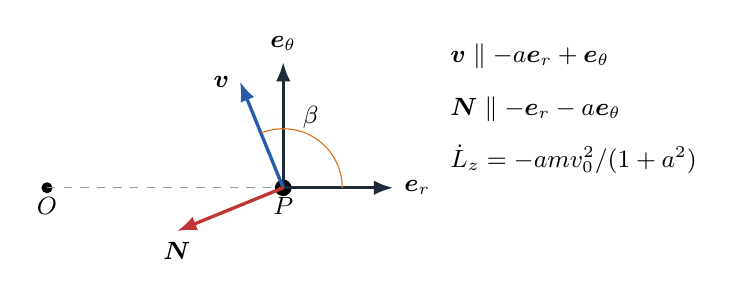
\begin{tikzpicture}[x=1cm,y=1cm,font=\small]

\fill (0,0) circle(2pt) node[below] {$O$};\fill (3,0) circle(3pt) node[below] {$P$};
\draw[guide] (0,0)--(4.4,0);\draw[axis] (3,0)--(4.4,0) node[right] {$\boldsymbol e_r$};
\draw[axis] (3,0)--(3,1.6) node[above] {$\boldsymbol e_\theta$};
\draw[vec] (3,0)--(2.45,1.35) node[left] {$\boldsymbol v$};
\draw[force] (3,0)--(1.65,-.55) node[below] {$\boldsymbol N$};
\draw[orange] (3.75,0) arc[start angle=0,end angle=112.2,radius=.75];\node at (3.35,.9) {$\beta$};
\node[align=left,anchor=west] at (5,1) {$\boldsymbol v\parallel-a\boldsymbol e_r+\boldsymbol e_\theta$\\[8pt] $\boldsymbol N\parallel-\boldsymbol e_r-a\boldsymbol e_\theta$\\[8pt] $\dot L_z=-amv_0^2/(1+a^2)$};

\end{tikzpicture}

% 5 question-03
\begin{tikzpicture}[x=1cm,y=1cm,font=\small]

\draw[body] (0,3)--(0,1) to[out=-90,in=180] (2,0)--(5,0) to[out=0,in=-90] (7,1)--(7,3);
\draw[blue,very thick] (3.5,0) ellipse (.3 and 1.05);
\fill[orange] (0,2.7) circle(4pt) node[left] {$m,q$};
\draw[dim] (-.65,0)--(-.65,2.7) node[midway,left] {$H$};
\draw[axis] (2.5,-1.5)--(5.5,-1.5) node[right] {$x$};
\node at (3.5,1.45) {一匝线圈，半径 $b$};
\node[align=left,anchor=west] at (8,1.5) {$a\ll b$\\[8pt] $R=2\rho b/a^2$\\[8pt] 仅线圈附近近似直轨道};

\end{tikzpicture}

% 6 solution-03
\begin{tikzpicture}[x=1cm,y=1cm,font=\small]
\draw[axis] (-3.5,0)--(3.5,0) node[right] {$x/b$};\draw[axis] (0,-2)--(0,2.2) node[above] {局部路径};\draw[body] (-3,0)--(3,0);\draw[blue,very thick] (0,0) ellipse (.25 and 1.2);

\fill[orange] (-1.6,0) circle(4pt);\draw[vec] (-1.6,.45)--(-.5,.45) node[above] {$v>0$};
\draw[force] (-1.6,-.35)--(-2.7,-.35) node[below] {$F_x<0$};
\node[align=left,anchor=west] at (4.4,1) {$F_x=-K^2v/[R(x^2+b^2)^3]$\\[8pt] $\Delta v=3\pi\mu_0^2q^2/(32mRb)$\\[8pt] 完整通过要求 $v_{\rm in}>\Delta v$\\[8pt] $K=\mu_0qb^2/2$};

\end{tikzpicture}

% 7 question-04
\begin{tikzpicture}[x=1cm,y=1cm,font=\small]

\draw[body,fill=blue!5] (0,0) rectangle (7,2);
\draw[body] (.8,-.3) circle(.25);\draw[body] (6.2,-.3) circle(.25);
\node at (1,1) {$T_l=300\,\mathrm K$};\node at (5.6,1) {$T_r=332\,\mathrm K$};
\draw[dim] (0,2.4)--(7,2.4) node[midway,above] {$L=10\,\mathrm m$};
\draw[axis] (0,-1)--(7.5,-1) node[right] {$x$};
\node at (3.5,-1.8) {容器与车 $M=150\,\mathrm{kg}$，气体 $m=120\,\mathrm{kg}$};

\end{tikzpicture}

% 8 solution-04
\begin{tikzpicture}[x=1cm,y=1cm,font=\small]
\draw[axis] (0,0)--(5.6,0) node[right] {$x/L$};\draw[axis] (0,0)--(0,3) node[above] {归一化量};
\draw[very thick,red] plot coordinates {(0.000000,2.000000) (0.128205,2.005470) (0.256410,2.010940) (0.384615,2.016410) (0.512821,2.021880) (0.641026,2.027350) (0.769231,2.032821) (0.897436,2.038291) (1.025641,2.043761) (1.153846,2.049231) (1.282051,2.054701) (1.410256,2.060171) (1.538462,2.065641) (1.666667,2.071111) (1.794872,2.076581) (1.923077,2.082051) (2.051282,2.087521) (2.179487,2.092991) (2.307692,2.098462) (2.435897,2.103932) (2.564103,2.109402) (2.692308,2.114872) (2.820513,2.120342) (2.948718,2.125812) (3.076923,2.131282) (3.205128,2.136752) (3.333333,2.142222) (3.461538,2.147692) (3.589744,2.153162) (3.717949,2.158632) (3.846154,2.164103) (3.974359,2.169573) (4.102564,2.175043) (4.230769,2.180513) (4.358974,2.185983) (4.487179,2.191453) (4.615385,2.196923) (4.743590,2.202393) (4.871795,2.207863) (5.000000,2.213333)};
\draw[very thick,blue] plot coordinates {(0.000000,2.000000) (0.128205,1.994545) (0.256410,1.989119) (0.384615,1.983723) (0.512821,1.978356) (0.641026,1.973019) (0.769231,1.967709) (0.897436,1.962429) (1.025641,1.957176) (1.153846,1.951952) (1.282051,1.946755) (1.410256,1.941586) (1.538462,1.936445) (1.666667,1.931330) (1.794872,1.926243) (1.923077,1.921182) (2.051282,1.916148) (2.179487,1.911140) (2.307692,1.906158) (2.435897,1.901202) (2.564103,1.896272) (2.692308,1.891368) (2.820513,1.886488) (2.948718,1.881634) (3.076923,1.876805) (3.205128,1.872000) (3.333333,1.867220) (3.461538,1.862464) (3.589744,1.857733) (3.717949,1.853025) (3.846154,1.848341) (3.974359,1.843681) (4.102564,1.839044) (4.230769,1.834431) (4.358974,1.829840) (4.487179,1.825273) (4.615385,1.820728) (4.743590,1.816206) (4.871795,1.811706) (5.000000,1.807229)};

\node[red,anchor=west] at (5.8,2.25) {$T/T_l$};
\node[blue,anchor=west] at (5.8,1.75) {$\rho(x)/\rho(0)$};
\node[align=left,anchor=west] at (7.9,1.9) {气体相对容器：向左\\[8pt] 容器位移 $X$：向右\\[8pt] $P=157.865\,\mathrm{atm}$};
\draw[vec] (1.7,-.8)--(.5,-.8) node[midway,below] {气体偏移};
\draw[vec] (3.3,-.8)--(4.5,-.8) node[midway,below] {容器位移};

\end{tikzpicture}

% 9 question-05
\begin{tikzpicture}[x=1cm,y=1cm,font=\small]
\draw[axis] (0,0)--(8.5,0) node[right] {$\theta/^\circ$};\draw[axis] (0,-2.4)--(0,2.4) node[above] {$\alpha/^\circ$};
\draw[very thick,blue] plot coordinates {(0.000000,0.000000) (1.000000,2.000000)};
\draw[very thick,blue] plot coordinates {(1.000000,-1.000000) (3.000000,1.000000)};
\draw[very thick,blue] plot coordinates {(3.000000,-2.000000) (5.000000,2.000000)};
\draw[very thick,blue] plot coordinates {(5.000000,-1.000000) (7.000000,1.000000)};
\draw[very thick,blue] plot coordinates {(7.000000,-2.000000) (8.000000,0.000000)};
\draw[guide] (1.0,-2.15)--(1.0,2.15);\node[below] at (1.0,-2.3) {$45$};
\draw[guide] (3.0,-2.15)--(3.0,2.15);\node[below] at (3.0,-2.3) {$135$};
\draw[guide] (5.0,-2.15)--(5.0,2.15);\node[below] at (5.0,-2.3) {$225$};
\draw[guide] (7.0,-2.15)--(7.0,2.15);\node[below] at (7.0,-2.3) {$315$};
\node[left] at (0,2) {$90$};\node[left] at (0,-2) {$-90$};\node at (4,-3.1) {原扫描折线的关键断点与有向角};
\end{tikzpicture}

% 10 solution-05
\begin{tikzpicture}[x=1.5cm,y=1.5cm,font=\small]
\draw[body] plot coordinates {(-1.000000,1.000000) (-0.977528,1.009204) (-0.955056,1.018198) (-0.932584,1.026983) (-0.910112,1.035559) (-0.887640,1.043926) (-0.865169,1.052084) (-0.842697,1.060032) (-0.820225,1.067772) (-0.797753,1.075302) (-0.775281,1.082623) (-0.752809,1.089735) (-0.730337,1.096638) (-0.707865,1.103331) (-0.685393,1.109815) (-0.662921,1.116091) (-0.640449,1.122157) (-0.617978,1.128013) (-0.595506,1.133661) (-0.573034,1.139100) (-0.550562,1.144329) (-0.528090,1.149349) (-0.505618,1.154160) (-0.483146,1.158762) (-0.460674,1.163154) (-0.438202,1.167338) (-0.415730,1.171312) (-0.393258,1.175077) (-0.370787,1.178633) (-0.348315,1.181980) (-0.325843,1.185118) (-0.303371,1.188046) (-0.280899,1.190765) (-0.258427,1.193275) (-0.235955,1.195576) (-0.213483,1.197668) (-0.191011,1.199550) (-0.168539,1.201224) (-0.146067,1.202688) (-0.123596,1.203943) (-0.101124,1.204989) (-0.078652,1.205826) (-0.056180,1.206453) (-0.033708,1.206871) (-0.011236,1.207081) (0.011236,1.207081) (0.033708,1.206871) (0.056180,1.206453) (0.078652,1.205826) (0.101124,1.204989) (0.123596,1.203943) (0.146067,1.202688) (0.168539,1.201224) (0.191011,1.199550) (0.213483,1.197668) (0.235955,1.195576) (0.258427,1.193275) (0.280899,1.190765) (0.303371,1.188046) (0.325843,1.185118) (0.348315,1.181980) (0.370787,1.178633) (0.393258,1.175077) (0.415730,1.171312) (0.438202,1.167338) (0.460674,1.163154) (0.483146,1.158762) (0.505618,1.154160) (0.528090,1.149349) (0.550562,1.144329) (0.573034,1.139100) (0.595506,1.133661) (0.617978,1.128013) (0.640449,1.122157) (0.662921,1.116091) (0.685393,1.109815) (0.707865,1.103331) (0.730337,1.096638) (0.752809,1.089735) (0.775281,1.082623) (0.797753,1.075302) (0.820225,1.067772) (0.842697,1.060032) (0.865169,1.052084) (0.887640,1.043926) (0.910112,1.035559) (0.932584,1.026983) (0.955056,1.018198) (0.977528,1.009204) (1.000000,1.000000)};
\draw[body] plot coordinates {(-1.000000,-1.000000) (-0.977528,-1.009204) (-0.955056,-1.018198) (-0.932584,-1.026983) (-0.910112,-1.035559) (-0.887640,-1.043926) (-0.865169,-1.052084) (-0.842697,-1.060032) (-0.820225,-1.067772) (-0.797753,-1.075302) (-0.775281,-1.082623) (-0.752809,-1.089735) (-0.730337,-1.096638) (-0.707865,-1.103331) (-0.685393,-1.109815) (-0.662921,-1.116091) (-0.640449,-1.122157) (-0.617978,-1.128013) (-0.595506,-1.133661) (-0.573034,-1.139100) (-0.550562,-1.144329) (-0.528090,-1.149349) (-0.505618,-1.154160) (-0.483146,-1.158762) (-0.460674,-1.163154) (-0.438202,-1.167338) (-0.415730,-1.171312) (-0.393258,-1.175077) (-0.370787,-1.178633) (-0.348315,-1.181980) (-0.325843,-1.185118) (-0.303371,-1.188046) (-0.280899,-1.190765) (-0.258427,-1.193275) (-0.235955,-1.195576) (-0.213483,-1.197668) (-0.191011,-1.199550) (-0.168539,-1.201224) (-0.146067,-1.202688) (-0.123596,-1.203943) (-0.101124,-1.204989) (-0.078652,-1.205826) (-0.056180,-1.206453) (-0.033708,-1.206871) (-0.011236,-1.207081) (0.011236,-1.207081) (0.033708,-1.206871) (0.056180,-1.206453) (0.078652,-1.205826) (0.101124,-1.204989) (0.123596,-1.203943) (0.146067,-1.202688) (0.168539,-1.201224) (0.191011,-1.199550) (0.213483,-1.197668) (0.235955,-1.195576) (0.258427,-1.193275) (0.280899,-1.190765) (0.303371,-1.188046) (0.325843,-1.185118) (0.348315,-1.181980) (0.370787,-1.178633) (0.393258,-1.175077) (0.415730,-1.171312) (0.438202,-1.167338) (0.460674,-1.163154) (0.483146,-1.158762) (0.505618,-1.154160) (0.528090,-1.149349) (0.550562,-1.144329) (0.573034,-1.139100) (0.595506,-1.133661) (0.617978,-1.128013) (0.640449,-1.122157) (0.662921,-1.116091) (0.685393,-1.109815) (0.707865,-1.103331) (0.730337,-1.096638) (0.752809,-1.089735) (0.775281,-1.082623) (0.797753,-1.075302) (0.820225,-1.067772) (0.842697,-1.060032) (0.865169,-1.052084) (0.887640,-1.043926) (0.910112,-1.035559) (0.932584,-1.026983) (0.955056,-1.018198) (0.977528,-1.009204) (1.000000,-1.000000)};

\draw[body] (-1,-1)--(-1,1);\draw[body] (1,-1)--(1,1);
\draw[axis] (-1.6,0)--(2,0) node[right] {$x$};\draw[axis] (0,-1.6)--(0,1.8) node[above] {$y$};
\fill (0,0) circle(2pt) node[below left] {$O$};
\draw[dim] (0,0)--(1,1) node[midway,left] {$r_0$};
\draw[ray] (3,0)--(1,0);\draw[ray] (1,0)--(2.7,0);
\node[below] at (1,-1) {$(d,-d)$};
\node[align=left,anchor=west] at (4,.8) {$d=r_0/\sqrt2$\\[8pt] $K=(1+\sqrt2)d$\\[8pt] 上帽：$y=(K^2-x^2)/(2K)$\\[8pt] 下帽：$y=-(K^2-x^2)/(2K)$};

\end{tikzpicture}

% 11 question-06
\begin{tikzpicture}[x=1cm,y=1cm,font=\small]

\draw[body,fill=blue!7] (0,0)--(0,3.5)--(5,0)--cycle;
\draw[body,fill=orange!8] (2.23,2.3) circle(.65);\node at (2.23,2.3) {$m$};
\node at (1.2,.7) {$M$};\draw[guide] (-.6,0)--(5.8,0);
\draw[orange] (4,0) arc[start angle=180,end angle=145,radius=1];\node at (3.7,.45) {$\theta$};
\draw[vec] (.9,-.65)--(-.2,-.65) node[midway,below] {$\ddot X$（自由时）};
\draw[vec] (3.2,1.8)--(4.3,1.03) node[right] {$\ddot s$};

\end{tikzpicture}

% 12 solution-06
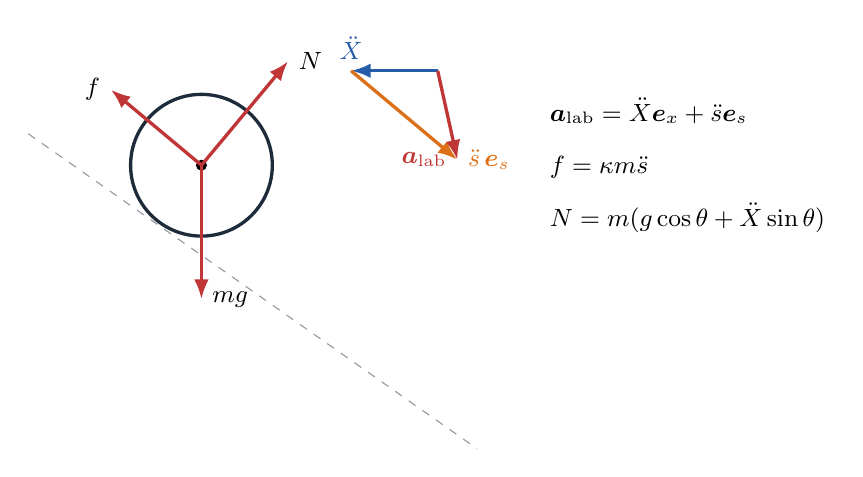
\begin{tikzpicture}[x=1cm,y=1cm,font=\small]

\draw[guide] (-1,1)--(4.7,-3);
\draw[body] (1.2,.6) circle(.9);\fill (1.2,.6) circle(2pt);
\draw[force] (1.2,.6)--(1.2,-1.1) node[right] {$mg$};
\draw[force] (1.2,.6)--(2.3,1.92) node[right] {$N$};
\draw[force] (1.2,.6)--(.05,1.56) node[left] {$f$};
\draw[vec,blue] (4.2,1.8)--(3.1,1.8) node[above] {$\ddot X$};
\draw[vec,orange] (3.1,1.8)--(4.45,.67) node[right] {$\ddot s\,\boldsymbol e_s$};
\draw[vec,red] (4.2,1.8)--(4.45,.67) node[left] {$\boldsymbol a_{\rm lab}$};
\node[align=left,anchor=west] at (5.5,.6) {$\boldsymbol a_{\rm lab}=\ddot X\boldsymbol e_x+\ddot s\boldsymbol e_s$\\[8pt] $f=\kappa m\ddot s$\\[8pt] $N=m(g\cos\theta+\ddot X\sin\theta)$};

\end{tikzpicture}

% 13 question-07
\begin{tikzpicture}[x=1cm,y=1cm,font=\small]

\draw[ray] (0,0)--(2,0) node[midway,above] {$\gamma$};
\node[mass] at (2.5,0) {$p$};
\draw[vec] (3,0)--(4.3,.8) node[right] {$K^+$};\draw[vec] (3,0)--(4.3,-.8) node[right] {$\Lambda^0$};
\begin{scope}[xshift=7cm]
\draw[vec] (0,0)--(1.5,0) node[midway,above] {$\beta c$};
\node at (-.5,0) {$\Lambda^0$};
\draw[vec] (1.6,0)--(3.2,.9) node[right] {$\pi^-$};
\draw[vec] (1.6,0)--(3.2,-.6) node[right] {$p$};
\end{scope}
\node at (5,-1.9) {反应阈值与飞行母粒子的两体衰变};

\end{tikzpicture}

% 14 solution-07
\begin{tikzpicture}[x=1cm,y=1cm,font=\small]
\draw[axis] (0,0)--(5.2,0) node[right] {$p_\parallel$};\draw[axis] (0,-1.9)--(0,1.9) node[above] {$p_\perp$};
\draw[body] plot coordinates {(4.432513,0.000000) (4.431022,0.047847) (4.426553,0.095619) (4.419113,0.143241) (4.408713,0.190640) (4.395370,0.237741) (4.379103,0.284472) (4.359940,0.330758) (4.337908,0.376527) (4.313044,0.421709) (4.285386,0.466232) (4.254977,0.510027) (4.221864,0.553026) (4.186099,0.595161) (4.147738,0.636367) (4.106842,0.676580) (4.063473,0.715736) (4.017699,0.753774) (3.969592,0.790636) (3.919228,0.826263) (3.866684,0.860600) (3.812043,0.893593) (3.755390,0.925191) (3.696813,0.955345) (3.636405,0.984007) (3.574259,1.011132) (3.510472,1.036679) (3.445144,1.060607) (3.378377,1.082879) (3.310275,1.103460) (3.240944,1.122318) (3.170493,1.139424) (3.099033,1.154751) (3.026673,1.168275) (2.953528,1.179974) (2.879711,1.189832) (2.805338,1.197831) (2.730525,1.203960) (2.655389,1.208210) (2.580046,1.210573) (2.504616,1.211046) (2.429215,1.209627) (2.353961,1.206321) (2.278971,1.201130) (2.204364,1.194065) (2.130254,1.185134) (2.056759,1.174354) (1.983993,1.161740) (1.912068,1.147311) (1.841099,1.131092) (1.771194,1.113106) (1.702465,1.093383) (1.635017,1.071952) (1.568957,1.048847) (1.504387,1.024105) (1.441408,0.997764) (1.380118,0.969865) (1.320614,0.940452) (1.262988,0.909570) (1.207330,0.877268) (1.153727,0.843596) (1.102263,0.808607) (1.053018,0.772356) (1.006069,0.734899) (0.961489,0.696294) (0.919347,0.656602) (0.879711,0.615884) (0.842641,0.574206) (0.808196,0.531630) (0.776428,0.488225) (0.747389,0.444057) (0.721122,0.399196) (0.697670,0.353711) (0.677069,0.307675) (0.659350,0.261158) (0.644543,0.214233) (0.632668,0.166973) (0.623747,0.119453) (0.617791,0.071747) (0.614811,0.023928) (0.614811,-0.023928) (0.617791,-0.071747) (0.623747,-0.119453) (0.632668,-0.166973) (0.644543,-0.214233) (0.659350,-0.261158) (0.677069,-0.307675) (0.697670,-0.353711) (0.721122,-0.399196) (0.747389,-0.444057) (0.776428,-0.488225) (0.808196,-0.531630) (0.842641,-0.574206) (0.879711,-0.615884) (0.919347,-0.656602) (0.961489,-0.696294) (1.006069,-0.734899) (1.053018,-0.772356) (1.102263,-0.808607) (1.153727,-0.843596) (1.207330,-0.877268) (1.262988,-0.909570) (1.320614,-0.940452) (1.380118,-0.969865) (1.441408,-0.997764) (1.504387,-1.024105) (1.568957,-1.048847) (1.635017,-1.071952) (1.702465,-1.093383) (1.771194,-1.113106) (1.841099,-1.131092) (1.912068,-1.147311) (1.983993,-1.161740) (2.056759,-1.174354) (2.130254,-1.185134) (2.204364,-1.194065) (2.278971,-1.201130) (2.353961,-1.206321) (2.429215,-1.209627) (2.504616,-1.211046) (2.580046,-1.210573) (2.655389,-1.208210) (2.730525,-1.203960) (2.805338,-1.197831) (2.879711,-1.189832) (2.953528,-1.179974) (3.026673,-1.168275) (3.099033,-1.154751) (3.170493,-1.139424) (3.240944,-1.122318) (3.310275,-1.103460) (3.378377,-1.082879) (3.445144,-1.060607) (3.510472,-1.036679) (3.574259,-1.011132) (3.636405,-0.984007) (3.696813,-0.955345) (3.755390,-0.925191) (3.812043,-0.893593) (3.866684,-0.860600) (3.919228,-0.826263) (3.969592,-0.790636) (4.017699,-0.753774) (4.063473,-0.715736) (4.106842,-0.676580) (4.147738,-0.636367) (4.186099,-0.595161) (4.221864,-0.553026) (4.254977,-0.510027) (4.285386,-0.466232) (4.313044,-0.421709) (4.337908,-0.376527) (4.359940,-0.330758) (4.379103,-0.284472) (4.395370,-0.237741) (4.408713,-0.190640) (4.419113,-0.143241) (4.426553,-0.095619) (4.431022,-0.047847) (4.432513,-0.000000)};
\draw[very thick,orange] plot coordinates {(0.000000,0.000000) (1.079267,0.792039)};
\fill (1.079267,0.792039) circle(2pt) node[above] {$\theta_{\max}\text{切点}$};
\fill (4.432513,0.000000) circle(2pt) node[below] {$p_{\max}$};
\node[align=left,anchor=west] at (6,1) {$p_{\max}=369.376\,\mathrm{MeV}/c$\\[8pt] $\theta_{\max}=36.274^\circ$\\[8pt] 最大动量与最大方向角位置不同};
\end{tikzpicture}

% 15 question-08
\begin{tikzpicture}[x=1cm,y=1cm,font=\small]

\draw[body] (0,0) circle(2.4);\draw[body] (0,0) circle(1.65);\draw[body] (0,0) circle(.72);
\draw[dim] (0,0)--(25:2.4) node[midway,above] {$r_1$};
\draw[dim] (0,0)--(145:1.65) node[midway,above] {$r_2$};
\draw[dim] (0,0)--(-60:.72) node[midway,left] {$r_3$};
\draw[body] (0,-.72)--(0,-3);\draw[body] (-.4,-3)--(.4,-3);\draw[body] (-.25,-3.15)--(.25,-3.15);
\node at (0,1.98) {$\varepsilon_{r1},\sigma_1$};\node at (0,1.13) {$\varepsilon_{r2},\sigma_2$};
\node[align=left,anchor=west] at (3.4,1) {外壳：$U>0$\\[8pt] 中壳：悬浮\\[8pt] 内壳：接地\\[8pt] 电流径向向内};

\end{tikzpicture}

% 16 solution-08
\begin{tikzpicture}[x=1cm,y=1cm,font=\small]

\node at (0,1.5) {$U$};\node at (3.5,1.5) {$V_2$};\node at (7,1.5) {$0$};
\draw[body] (0,1.1)--(0,0)--(.5,0);\draw[resistor] (.5,0)--(3,0);\draw[body] (3,0)--(4,0);
\draw[resistor] (4,0)--(6.5,0);\draw[body] (6.5,0)--(7,0)--(7,1.1);
\node[below] at (1.75,0) {$R_1$};\node[below] at (5.25,0) {$R_2$};
\draw[current] (.8,.7)--(2.6,.7) node[midway,above] {$I$};
\draw[current] (4.4,.7)--(6.2,.7) node[midway,above] {$I$};
\draw[body] (0,0)--(0,-1.3)--(1.5,-1.3);\draw[body] (2,-1.3)--(3.5,-1.3)--(3.5,0);
\draw[body] (1.5,-1.65)--(1.5,-.95);\draw[body] (2,-1.65)--(2,-.95);
\node[below] at (1.75,-1.8) {$C_1$};
\draw[body] (3.5,-1.3)--(5,-1.3);\draw[body] (5.5,-1.3)--(7,-1.3)--(7,0);
\draw[body] (5,-1.65)--(5,-.95);\draw[body] (5.5,-1.65)--(5.5,-.95);\node[below] at (5.25,-1.8) {$C_2$};
\node[align=left,anchor=west] at (8.3,.3) {$q_{1,\rm inner}=\varepsilon_0I/\sigma_1$\\[8pt] $q_{f2}=\varepsilon_0I(\varepsilon_{r2}/\sigma_2-\varepsilon_{r1}/\sigma_1)$\\[8pt] 稳态由电阻分压决定};

\end{tikzpicture}
\end{document}
